% Flowing English fragments: source-frame markers never force a page break.
% Integration requirements: amsmath, amssymb, graphicx, tikz and tikz-cd.
\providecommand{\EnglishSourceFrame}[2]{\par\smallskip\noindent{\footnotesize\texttt{#1} [source label: #2]}\par\smallskip}
\providecommand{\EnglishUnclear}[3]{\textit{[unclear #1/#2: #3]}}
\providecommand{\EnglishIncomplete}[3]{\textit{[undeciphered #1/#2: #3]}}
\providecommand{\EnglishSourceFigure}[3]{\par\noindent\textit{Source detail #1/#2: #3}\par}
\EnglishSourceFrame{GELFAND-P001349}{unlabelled}
\underline{2/III--87}\qquad \underline{V. Kazakov.}
\underline{The problem of gluing surfaces of genus $g$ from a $2n$-gon.}

\EnglishDiagramPair{GELFAND-P001349}{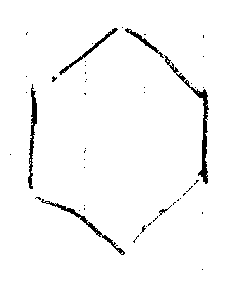
\includegraphics[width=.98\linewidth,height=45mm,keepaspectratio]{english/reader-working/chapter29-batch01/figures/gelfand-0146-d02-gelfand-p001349-original.png}}{
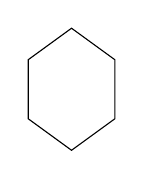
\begin{tikzpicture}[x=1cm,y=1cm]
\draw (0,0.6)--(0.55,1)--(1.1,0.6)--(1.1,-0.15)--(0.55,-0.55)--(0,-0.15)--cycle;
\end{tikzpicture}
}
\par\noindent\textit{Typed diagram explanation: the source draws an unlabelled polygon for the $2n$-gon; it supplies no additional side labels.}\par

$2n$-gon; gluing \EnglishUnclear{GELFAND-P001349}{header-hook}{check mark / $\gamma$}
\EnglishUnclear{GELFAND-P001349}{opposite-word}{oppos.? / opposite?} oriented sides (in pairs).

$g$ is the genus of the resulting manifold.
How many different ways yield a surface of genus $g$?
$f_n^g$ is the number of such ways of gluing.

(Some gluings may be forbidden.
\underline{Prohibitions:} 1)
\EnglishDiagramPair{GELFAND-P001349}{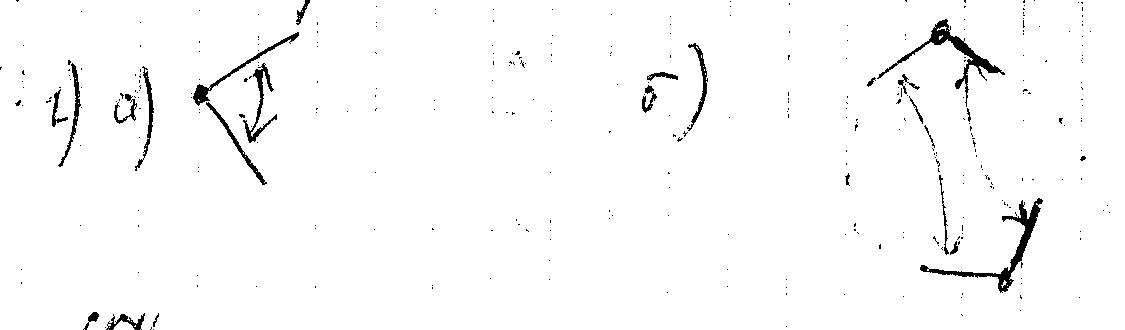
\includegraphics[width=.98\linewidth,height=45mm,keepaspectratio]{english/reader-working/chapter29-batch01/figures/gelfand-0146-d03-gelfand-p001349-original.png}}{
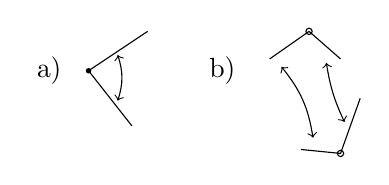
\begin{tikzpicture}[x=1cm,y=1cm]
\node at (-0.5,0) {a)};
\draw (0,0)--(0.75,0.5); \draw (0,0)--(0.55,-0.7);
\fill (0,0) circle (0.035);
\draw[<->] (0.37,0.2) to[bend left=18] (0.37,-0.38);
\node at (1.7,0) {b)};
\draw (2.3,0.15)--(2.8,0.5)--(3.2,0.15);
\draw (2.8,0.5) circle (0.04);
\draw (2.7,-1)--(3.2,-1.05)--(3.45,-0.35);
\draw (3.2,-1.05) circle (0.04);
\draw[<->] (2.45,0.05) to[bend left=15] (2.85,-0.85);
\draw[<->] (3.02,0.1) to[bend right=8] (3.25,-0.65);
\end{tikzpicture}
}
\par\noindent\textit{Typed diagram explanation: a) shows two sides meeting at a marked vertex; b) shows two separate marked vertices with two pairing arrows. The restrictions refer to these labelled local configurations.}\par

2) [Crossed out: OR] Only b) is forbidden.\qquad 3) Only a) is forbidden.

Everything reduces to the case without prohibitions.)



\par\smallskip\noindent\textit{Reading notes.}\par
\noindent\texttt{GELFAND-0146-U005} (header-hook): A single tall hook between “gluing” and the abbreviation for “opposite”; a separate mark.\par
Candidates: check mark; gamma. Unresolved in the frozen transcription.\par
\noindent\texttt{GELFAND-0146-U006} (opposite-word): An abbreviated word beginning “protivo...” (“oppos...”), with a full stop and a compressed ending.\par
Candidates: oppos.; opposite (abbreviated). Unresolved in the frozen transcription.\par
The two abbreviations for “opposite” do not settle whether an expanded phrase should refer to opposite sides or opposite orientation. Their source qualification is preserved.\par


\EnglishSourceFrame{GELFAND-P001350}{85}
Generating function:
\begin{equation*}
(1)\quad f_n(N)=\text{\EnglishUnclear{GELFAND-P001350}{sum-prefix}{one crossed-out symbol}}\sum_{g=0}^{\infty}N^{-2g}f_n^g.
\end{equation*}
Then
\begin{equation*}
(2)\quad f_n(N)=(2\pi)^{-N^2/2}\int d^{N^2}\varphi\,\frac{\operatorname{tr}}{N}(\varphi^{2n})e^{-N\operatorname{tr}\varphi^2/2}
=\left\langle\frac{\operatorname{tr}}{N}\varphi^{2n}\right\rangle,
\end{equation*}
where $\varphi^+=\varphi$ is an $N\times N$ Hermitian matrix.
\EnglishDiagramPair{GELFAND-P001350}{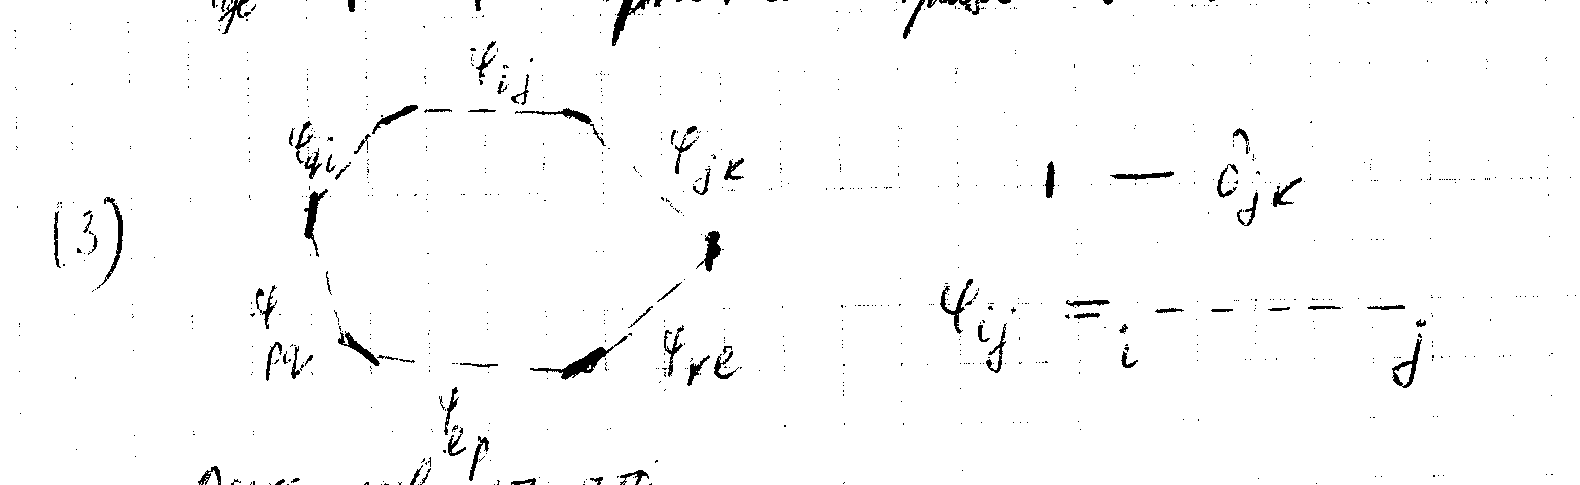
\includegraphics[width=.98\linewidth,height=45mm,keepaspectratio]{english/reader-working/chapter29-batch01/figures/gelfand-0146-d04-gelfand-p001350-original.png}}{
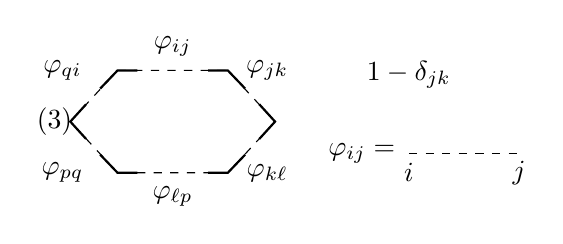
\begin{tikzpicture}[x=1cm,y=1cm]
\node at (-1.5,0) {(3)};
\draw[dashed] (-0.7,0.65)--(0.7,0.65)--(1.3,0)--(0.7,-0.65)--(-0.7,-0.65)--(-1.3,0)--cycle;
\draw[thick] (-0.92,0.42)--(-0.7,0.65)--(-0.45,0.65);
\draw[thick] (0.45,0.65)--(0.7,0.65)--(0.92,0.42);
\draw[thick] (1.1,0.22)--(1.3,0)--(1.1,-0.22);
\draw[thick] (0.92,-0.42)--(0.7,-0.65)--(0.45,-0.65);
\draw[thick] (-0.45,-0.65)--(-0.7,-0.65)--(-0.92,-0.42);
\draw[thick] (-1.1,-0.22)--(-1.3,0)--(-1.1,0.22);
\node at (0,0.95) {$\varphi_{ij}$}; \node at (1.2,0.65) {$\varphi_{jk}$};
\node at (1.2,-0.65) {$\varphi_{k\ell}$}; \node at (0,-0.95) {$\varphi_{\ell p}$};
\node at (-1.4,-0.65) {$\varphi_{pq}$}; \node at (-1.4,0.65) {$\varphi_{qi}$};
\node at (3.0,0.6) {$1-\delta_{jk}$};
\node at (2.4,-0.4) {$\varphi_{ij}=$}; \draw[dashed] (3,-0.4)--(4.4,-0.4);
\node at (3,-0.65) {$i$}; \node at (4.4,-0.65) {$j$};
\end{tikzpicture}
}
\par\noindent\textit{Typed diagram explanation: (3) writes the cyclic matrix entries around the polygon and represents $\varphi_{ij}$ by a dashed segment with endpoint labels $i,j$. The admitted written label is $1-\delta_{jk}$.}\par

It is easy to check that
\begin{equation*}
(4)\quad \langle\varphi_{ij}\varphi_{k\ell}\rangle=\frac1N\delta_{i\ell}\delta_{jk},
\end{equation*}
or
\EnglishDiagramPair{GELFAND-P001350}{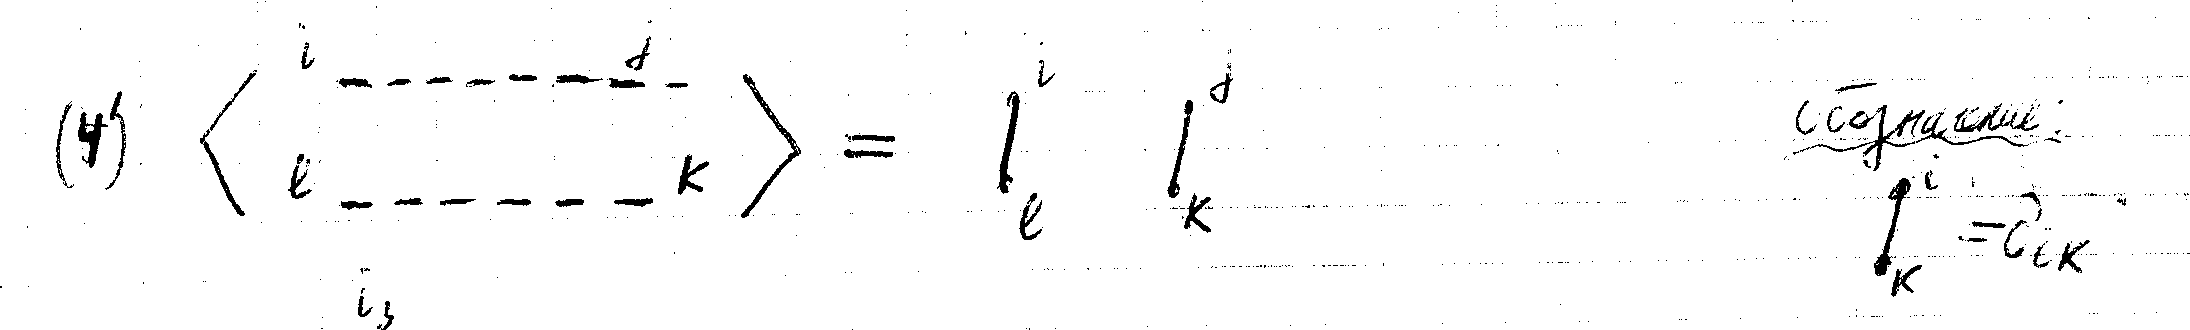
\includegraphics[width=.98\linewidth,height=45mm,keepaspectratio]{english/reader-working/chapter29-batch01/figures/gelfand-0146-d05-gelfand-p001350-original.png}}{
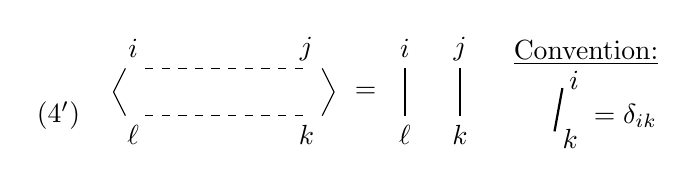
\begin{tikzpicture}[x=1cm,y=1cm]
\node at (-0.7,0) {$(4')$};
\draw (0.15,0.6)--(0,0.3)--(0.15,0); \draw (2.65,0.6)--(2.8,0.3)--(2.65,0);
\draw[dashed] (0.4,0.6)--(2.4,0.6); \draw[dashed] (0.4,0)--(2.4,0);
\node at (0.25,0.85) {$i$}; \node at (2.45,0.85) {$j$};
\node at (0.25,-0.25) {$\ell$}; \node at (2.45,-0.25) {$k$};
\node at (3.2,0.3) {$=$}; \draw[thick] (3.7,0.6)--(3.7,0); \draw[thick] (4.4,0.6)--(4.4,0);
\node at (3.7,0.85) {$i$}; \node at (3.7,-0.25) {$\ell$}; \node at (4.4,0.85) {$j$}; \node at (4.4,-0.25) {$k$};
\node at (6,0.8) {\underline{Convention:}};
\draw[thick] (5.7,0.35)--(5.6,-0.2); \node at (5.85,0.45) {$i$}; \node at (5.8,-0.3) {$k$}; \node at (6.5,0) {$=\delta_{ik}$};
\end{tikzpicture}
}
\par\noindent\textit{Typed diagram explanation: (4') identifies endpoint indices in the two pairings. The written caption is ``Convention'', and the segment with labels $i,k$ is assigned $\delta_{ik}$.}\par

\EnglishDiagramPair{GELFAND-P001350}{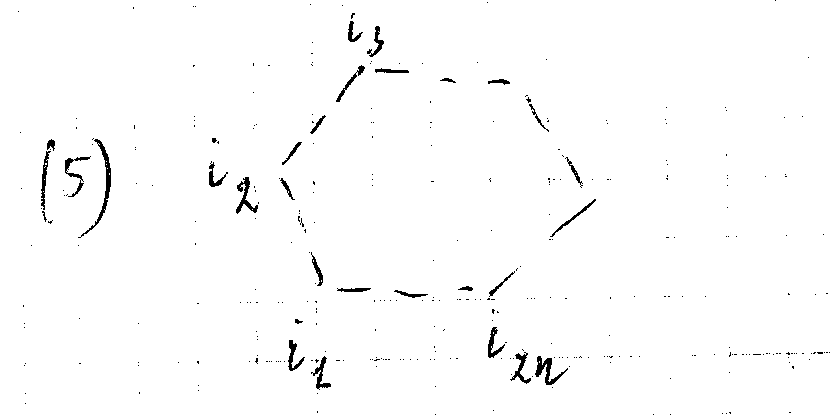
\includegraphics[width=.98\linewidth,height=45mm,keepaspectratio]{english/reader-working/chapter29-batch01/figures/gelfand-0146-d06-gelfand-p001350-original.png}}{
\begin{tikzpicture}[x=1cm,y=1cm]
\node at (-1.6,0) {(5)};
\draw[dashed] (-0.6,0.7)--(0.6,0.7)--(1.2,0)--(0.6,-0.7)--(-0.6,-0.7)--(-1.2,0)--cycle;
\node at (-0.65,0.95) {$i_3$}; \node at (-1.5,0) {$i_2$};
\node at (-0.65,-1) {$i_1$}; \node at (0.65,-1) {$i_{2n}$};
\end{tikzpicture}
}
\par\noindent\textit{Typed diagram explanation: (5) shows the polygon with indices $i_1,i_2,i_3,i_{2n}$; no missing intermediate labels are supplied.}\par

(6) \underline{Wick's theorem:} Let there be $2n$ Gaussian variables $\xi_1,\xi_2,\ldots,\xi_{2n}$. Then
([Crossed-out writing: \EnglishIncomplete{GELFAND-P001350}{wick-word}{short crossed-out writing under dense strokes; its exact reading has not been established}] [Inserted above: linear] functions of $\varphi_{ik}$)
\begin{equation*}
\langle\xi_1\xi_2\cdots\xi_{2n}\rangle
=\sum_{P(i_1,\ldots,i_{2n})}\langle\xi_{i_1}\xi_{i_2}\rangle\langle\xi_{i_3}\xi_{i_4}\rangle\cdots.
\end{equation*}
[Crossed out beneath the sum: \EnglishIncomplete{GELFAND-P001350}{cancel-index-first}{a short earlier line of indices; the initial index resembles $i_2$, but the reading has not been established}.]
Permutations [crossed out: $i_1,i_2,\ldots,i_{2n}$] $1,2,\ldots,2n$.
The sum is over all partitions into pairs.
\EnglishDiagramPair{GELFAND-P001350}{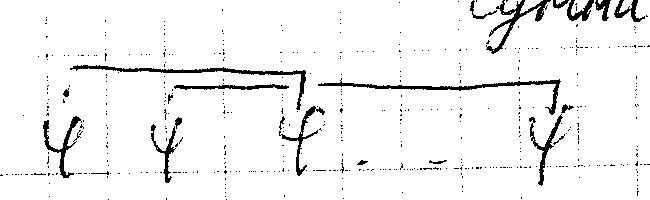
\includegraphics[width=.98\linewidth,height=45mm,keepaspectratio]{english/reader-working/chapter29-batch01/figures/gelfand-0146-d07-gelfand-p001350-original.png}}{
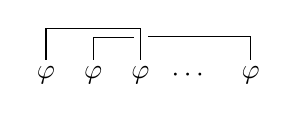
\begin{tikzpicture}[x=1cm,y=1cm]
\node at (0,0) {$\varphi$}; \node at (0.6,0) {$\varphi$}; \node at (1.2,0) {$\varphi$}; \node at (2.6,0) {$\varphi$};
\node at (1.8,0) {$\cdots$};
\draw (0,0.2)--(0,0.6)--(1.2,0.6)--(1.2,0.2);
\draw (0.6,0.2)--(0.6,0.48)--(1.12,0.48);
\draw (1.3,0.5)--(2.6,0.5)--(2.6,0.2);
\end{tikzpicture}
}
\par\noindent\textit{Typed diagram explanation: brackets join the displayed $\varphi$ symbols in pairs. This is an example of the pairings in the written Wick formula; it does not add another pairing rule.}\par

(\underline{Exercise}: \EnglishUnclear{GELFAND-P001350}{exercise-word}{to prove? / to render? / prove (imperative)? / render (imperative)?})

A more general theorem: let $\xi$ be a Gaussian variable; then
\begin{equation*}
(7)\quad \langle\xi f(\xi)\rangle=\langle\xi\xi\rangle\left\langle\frac{\partial f}{\partial\xi}\right\rangle.
\end{equation*}
\begin{equation*}
(8)\quad \langle\xi_i f(\xi)\rangle=\sum_j\langle\xi_i\xi_j\rangle\left\langle\frac{\partial f}{\partial\xi_j}\right\rangle.
\end{equation*}



\par\smallskip\noindent\textit{Reading notes.}\par
\noindent\texttt{GELFAND-0146-U007} (sum-prefix): One symbol between the equality sign and the sum in (1) is densely crossed out.\par
Candidates: none. Unresolved in the frozen transcription.\par
\noindent\texttt{GELFAND-0146-U008} (wick-word): Short densely crossed-out writing beneath the inserted word “linear”, before “functions of phi\_ik”; the exact letters have not been established.\par
Candidates: none. Unresolved in the frozen transcription.\par
The localized cancelled writing remains undeciphered. The frozen source frame remains partly unreadable; translating this note does not decipher the missing writing.\par
\noindent\texttt{GELFAND-0146-U009} (cancel-index-first): A short earlier line of indices beneath the sum is covered by several strokes; the first index resembles i\_2, but has not been read reliably.\par
Candidates: initial i\_2?. Unresolved in the frozen transcription.\par
The localized cancelled writing remains undeciphered. The frozen source frame remains partly unreadable; translating this note does not decipher the missing writing.\par
\noindent\texttt{GELFAND-0146-U036} (exercise-word): After “Exercise”, there is an initial loop with a fine arc, a middle “kaz...” and joined final strokes. The initial letter and the ending “at” (infinitive) versus “ite” (imperative) have not been reliably established.\par
Candidates: to prove; to render; prove (imperative); render (imperative). Unresolved in the frozen transcription.\par


\EnglishSourceFrame{GELFAND-P001351}{unlabelled}
Using (7) and (8), it is easy to prove \underline{Wick's theorem}
(\EnglishUnclear{GELFAND-P001351}{induction-word}{having used? by the number of $\xi$ variables?}).
\EnglishDiagramPair{GELFAND-P001351}{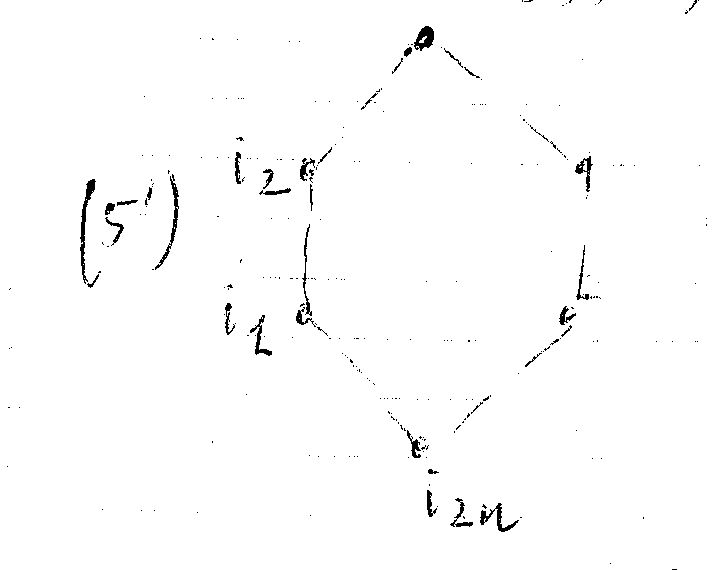
\includegraphics[width=.98\linewidth,height=45mm,keepaspectratio]{english/reader-working/chapter29-batch01/figures/gelfand-0146-d08-gelfand-p001351-original.png}}{
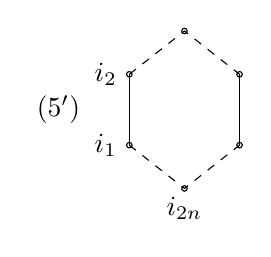
\begin{tikzpicture}[x=1cm,y=1cm]
\node at (-1.6,0) {$(5')$};
\draw[dashed] (-0.7,0.45)--(0,1)--(0.7,0.45);
\draw[dashed] (-0.7,-0.45)--(0,-1)--(0.7,-0.45);
\draw (-0.7,0.45)--(-0.7,-0.45); \draw (0.7,0.45)--(0.7,-0.45);
\draw (0,1) circle (0.035); \draw (0,-1) circle (0.035);
\draw (-0.7,0.45) circle (0.035); \draw (-0.7,-0.45) circle (0.035);
\draw (0.7,0.45) circle (0.035); \draw (0.7,-0.45) circle (0.035);
\node at (-1,0.45) {$i_2$}; \node at (-1,-0.45) {$i_1$}; \node at (0,-1.25) {$i_{2n}$};
\end{tikzpicture}
}
\par\noindent\textit{Typed diagram explanation: (5') marks polygon vertices and retains the written labels $i_1,i_2,i_{2n}$.}\par

We shall evaluate integral (2) using Wick's theorem. Clearly,
\begin{equation*}
(9)\quad \langle\operatorname{tr}\varphi^{2n}\rangle=
\langle\varphi_{i_1i_2}\varphi_{i_2i_3}\cdots\varphi_{i_{2n}i_1}\rangle.
\end{equation*}
[Crossed out between the equality sign and the bracket: $\sum$.]
Now apply Wick's theorem.
According to it, the sides must be paired! (Those of polygon $(5')$.)

Gluing.
\EnglishDiagramPair{GELFAND-P001351}{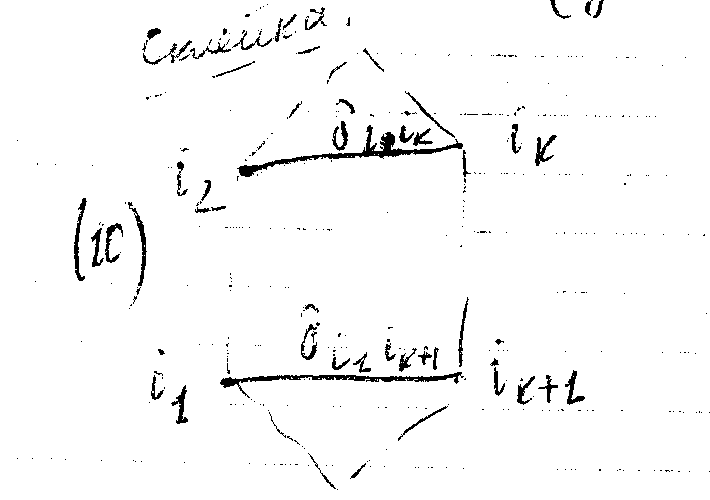
\includegraphics[width=.98\linewidth,height=45mm,keepaspectratio]{english/reader-working/chapter29-batch01/figures/gelfand-0146-d09-gelfand-p001351-original.png}}{
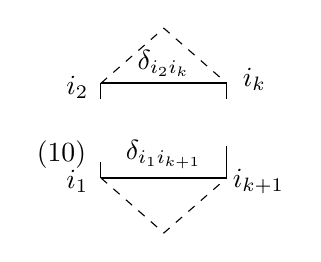
\begin{tikzpicture}[x=1cm,y=1cm]
\node at (-1.3,0) {(10)};
\draw[dashed] (-0.8,0.9)--(0,1.6)--(0.8,0.9); \draw[thick] (-0.8,0.9)--(0.8,0.9);
\draw (-0.8,0.9)--(-0.8,0.7); \draw (0.8,0.9)--(0.8,0.7);
\node at (-1.1,0.85) {$i_2$}; \node at (1.15,0.95) {$i_k$}; \node at (0,1.15) {$\delta_{i_2i_k}$};
\draw[thick] (-0.8,-0.3)--(0.8,-0.3);
\draw (-0.8,-0.3)--(-0.8,-0.1); \draw (0.8,-0.3)--(0.8,0.1);
\draw[dashed] (-0.8,-0.3)--(0,-1)--(0.8,-0.3);
\node at (-1.1,-0.35) {$i_1$}; \node at (1.2,-0.35) {$i_{k+1}$}; \node at (0,0) {$\delta_{i_1i_{k+1}}$};
\end{tikzpicture}
}
\par\noindent\textit{Typed diagram explanation: (10) pairs the upper endpoints $i_2,i_k$ and the lower endpoints $i_1,i_{k+1}$, with written Kronecker symbols $\delta_{i_2i_k}$ and $\delta_{i_1i_{k+1}}$.}\par

[Crossed out to the right of (10): $\varphi$ \EnglishUnclear{GELFAND-P001351}{cancel-phi}{an unreadable second crossed-out symbol}.]
$\varphi$-s (4) ensure the correct orientation in gluing
(because of Hermiticity!!)
(Choosing the matrix differently can yield a nonorientable surface.)
\EnglishDiagramPair{GELFAND-P001351}{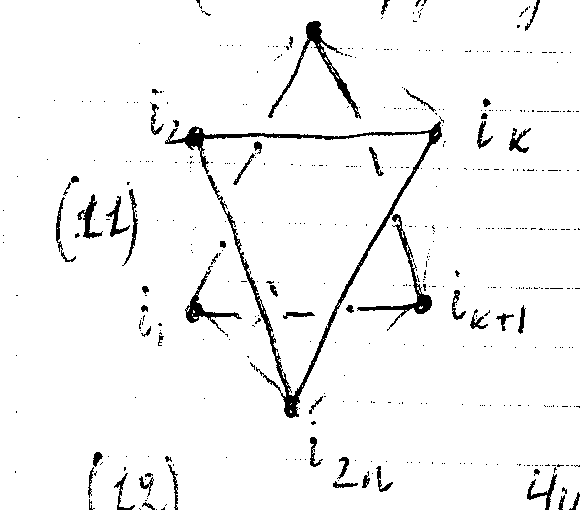
\includegraphics[width=.98\linewidth,height=45mm,keepaspectratio]{english/reader-working/chapter29-batch01/figures/gelfand-0146-d10-gelfand-p001351-original.png}}{
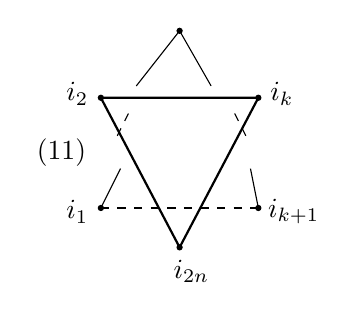
\begin{tikzpicture}[x=1cm,y=1cm]
\node at (-1.5,0) {(11)};
\draw[thick] (-1,0.7)--(1,0.7)--(0,-1.2)--cycle;
\fill (-1,0.7) circle (0.04); \fill (1,0.7) circle (0.04); \fill (0,-1.2) circle (0.04);
\draw (-0.55,0.85)--(0,1.55)--(0.4,0.85); \fill (0,1.55) circle (0.04);
\draw[dashed] (-0.65,0.5)--(-0.8,0.2); \draw[dashed] (0.7,0.5)--(0.85,0.2);
\draw (-0.75,-0.2)--(-1,-0.7); \draw (0.9,-0.2)--(1,-0.7);
\draw[dashed] (-1,-0.7)--(1,-0.7); \fill (-1,-0.7) circle (0.04); \fill (1,-0.7) circle (0.04);
\node at (-1.3,0.75) {$i_2$}; \node at (1.3,0.75) {$i_k$};
\node at (-1.3,-0.75) {$i_1$}; \node at (1.45,-0.75) {$i_{k+1}$}; \node at (0.15,-1.5) {$i_{2n}$};
\end{tikzpicture}
}
\par\noindent\textit{Typed diagram explanation: (11) illustrates the index loops after gluing. The surrounding lecture text assigns $N$ to each closed cycle.}\par

Closed loops $\longrightarrow$ a property of the Kronecker symbol,
that is, always $N$! For example,
\begin{equation*}
N=\delta_{i_2i_k}\,\delta_{i_ki_{2n}}\,\delta_{i_{2n}i_2}.
\end{equation*}
$\forall$ closed cycle gives $N$!

(12) \underline{Number of closed cycles = number of vertices in the glued closed figure.}

(13) The contribution of each possible gluing (diagram)
\begin{equation*}
=N^{-(\#\text{ edges})+(\#\text{ vertices})-1}=N^{-2g}.
\end{equation*}
(because of $\frac N2\operatorname{tr}\varphi^2$ in $\exp$)



\par\smallskip\noindent\textit{Reading notes.}\par
\noindent\texttt{GELFAND-0146-U010} (induction-word): In the upper parenthesis, a long word visibly begins “vospolz...” (“having used...”), followed by “by” and an unidentified final word. The letters do not confirm “by induction”.\par
Candidates: having used? by the number of xi’s?. Unresolved in the frozen transcription.\par
\noindent\texttt{GELFAND-0146-U011} (cancel-phi): To the right of (10), a short crossed-out group has two symbols. The first resembles phi; the second is elongated and overlapped by diagonal strokes.\par
Candidates: phi and a second unidentified symbol. Unresolved in the frozen transcription.\par
The letters do not establish “by induction”. The translation retains the candidate wording without supplying a proof method.\par


\EnglishSourceFrame{GELFAND-P001352}{86}
We shall evaluate integral (2). Reduce it to \EnglishUnclear{GELFAND-P001352}{header-word}{diag.? / sym.? / eig.?} form:
\begin{equation*}
(14)\quad \varphi_{ij}=\sum_k\Omega^+_{ik}\lambda_k\Omega_{kj},\qquad \Omega\text{ is a unitary matrix}.
\end{equation*}
\begin{equation*}
(15)\quad d^{N^2}\varphi=\left(\prod d\lambda_i\,[\Delta(\lambda)]^2\right)d\Omega,
\end{equation*}
where
\begin{equation*}
\Delta(\lambda)=\prod_{i>j}(\lambda_i-\lambda_j).
\end{equation*}
[Crossed-out number on the left: \EnglishUnclear{GELFAND-P001352}{cancel-number}{$(14)$ / $(16)$}.]
[Boxed on the right: See H. \underline{Weyl}: The Classical Groups: Their Invariants and Representations]
(Dyson measure).

([Above the start of the list: Brezin(?)], Itzykson, Zuber, \underline{Parisi},)
[A line descends from Parisi:] \underline{the stochastic quantization method}

quantum quantity $\longmapsto$ Markov process.
The mean is calculated by averaging over trajectories.
[On the left: works here. An arrow points down to (16).]
\begin{equation*}
\begin{aligned}
(16)\quad f_n(N)&\sim\int\prod\left(d\lambda_i\,e^{-N\lambda_i^2/2}\right)\Delta^2(\lambda)
\left(\frac1N\sum_{i=1}^{N}\lambda_i^{2n}\right)=\\
&=\text{\EnglishUnclear{GELFAND-P001352}{cancel-prefactor}{one crossed-out symbol before the integral}}
\int\prod\left(d\lambda_i\,e^{-N\lambda_i^2/2}\right)\Delta^2(\lambda)\lambda_1^{2n}\\
&\sim\int\prod\left(d\lambda_i\,e^{-\lambda_i^2/2}\right)\Delta^2(\lambda)\lambda_1^{2n}.
\end{aligned}
\end{equation*}
[A line descends from the second equality: symmetric in $\lambda_j$.]
(change of $\lambda_i$: take out \EnglishUnclear{GELFAND-P001352}{cancel-rescale}{one crossed-out symbol} $\sqrt N$ in $\lambda_i$)
\begin{equation*}
(17)\quad \Delta(\lambda)=\det\|(\lambda_\ell)^k\|_{k,\ell}=\det\|H_k(\lambda_\ell)\|.
\end{equation*}
$H_k$ is any polynomial of degree $k$ with leading coefficient $1$.
Choose the $H_k$ to be Hermite polynomials!!
(with a suitable scaling so that the leading coefficient $=1$)
(good, since $H_k$ and $H_\ell$ are orthogonal)

Hence:
\begin{equation*}
(18)\quad f_n(N)\sim\frac1C\int\prod_{i=1}^{N}\left(d\lambda_i\,e^{-\lambda_i^2/2}\right)\lambda_1^{2n}
\left[\sum_p\prod_{k=1}^{N}H_k(\lambda_{p_k})(-1)^{\operatorname{sgn}(p)}\right]^2=
\end{equation*}
[Beneath $p$: permutation.]
(Parisi and Bessis devised the technique with Hermite polynomials)
On squaring: $\forall$ variable $\lambda_{p_k}$ occurs exactly $2$ times.



\par\smallskip\noindent\textit{Reading notes.}\par
\noindent\texttt{GELFAND-0146-U012} (cancel-number): An earlier number before Delta(lambda) is crossed out.\par
Candidates: (14); (16). Unresolved in the frozen transcription.\par
\noindent\texttt{GELFAND-0146-U013} (cancel-prefactor): One elongated symbol before the second integral in (16) is crossed out.\par
Candidates: integral sign; 1. Unresolved in the frozen transcription.\par
\noindent\texttt{GELFAND-0146-U014} (cancel-rescale): One symbol before sqrt(N), in the parenthesis about changing lambda\_i, is densely crossed out.\par
Candidates: none. Unresolved in the frozen transcription.\par
\noindent\texttt{GELFAND-0146-U015} (header-word): A short abbreviation before “form”: its first strokes and ending resemble “diag.”, but the final reading has not been established.\par
Candidates: diag.; sym.; eig.. Unresolved in the frozen transcription.\par


\EnglishSourceFrame{GELFAND-P001353}{unlabelled}
\begin{equation*}
=\sum_{k=0}^{N-1}\frac{\int d\lambda\,e^{-\lambda^2}[H_k(\lambda)]^2\lambda^{2k}}
{\int d\lambda\,e^{-\lambda^2}(H_k(\lambda))^2}.
\end{equation*}
From a handbook (for example, Abramowitz):
\begin{equation*}
(19)\quad \int d\lambda\,e^{i\lambda x}e^{-\lambda^2}[H_k(\lambda)]^2
=\underbrace{\sqrt\pi\,2^n n!}_{\text{will cancel with the denominator}}
e^{-x^2/4}\underbrace{L_n(x^2/2)}_{\text{Laguerre polynomial}}.
\end{equation*}
Finally we obtain [arrow to (20)]:
\begin{equation*}
(20)\quad \sum_{n=0}^{\infty}\frac{(-x^2/2)^n}{(2n)!!}f_n(N)
=e^{-x^2/4}\sum_{i=0}^{N-1}L_i(x^2/2)
=e^{-x^2/4}\underbrace{L^1_{N-1}(x^2/2)}_{\text{associated Laguerre polynomials}}.
\end{equation*}
Here we \EnglishUnclear{GELFAND-P001353}{asympt-word}{most? / are interested in?} the asymptotics as $N\to\infty$. Form the generating function:
[Crossed out before (21): $F(x,t)$\EnglishUnclear{GELFAND-P001353}{cancel-21}{a final single symbol}.]
\begin{equation*}
(21)\quad f_n(t)=\sum_N t^N f_n(N).
\end{equation*}
The answer for it is:
\begin{equation*}
(22)\quad f_n(t)=\frac{(2n)!}{n!}\frac{(t+1)^n}{(1-t)^{n+2}}.
\end{equation*}
We are interested in the expansion as a \underline{series} in \underline{$t$}.
\underline{Zakharevich: answer (according to D. Zagier)}
\begin{equation*}
(23)\quad \sum_{g=0}^{\infty}\frac{(n+1)!(n-2g)!}{(2n)!}\,f_g^n x^g
=\left(\frac{\sqrt{x/2}}{\operatorname{th}\sqrt{x/2}}\right)^{n+1}.
\end{equation*}
[Separately in the left margin: (]
(when $n-2g<0$, multiply by $(2n)!$ and transfer to the right-hand side)
$f_g^n(n-2g)!$ is thereby defined also when $2g>n$(!).

\underline{Variant:}
\underline{2 other combinatorial problems} (considered by Kazakov and Migdal).
\tikz{\node[draw,circle,inner sep=1pt] {1};} How to tile a $2n$-gon with $k$ triangles so that the resulting surface has genus $g$.
[Crossed-out line: Number \EnglishUnclear{GELFAND-P001353}{cancel-variant-line}{gluings?}.]
\EnglishDiagramPair{GELFAND-P001353}{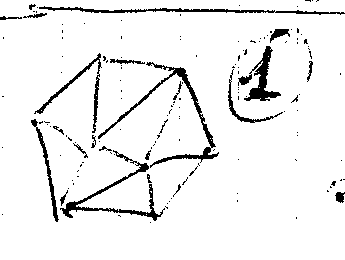
\includegraphics[width=.98\linewidth,height=45mm,keepaspectratio]{english/reader-working/chapter29-batch01/figures/gelfand-0146-d11-gelfand-p001353-original.png}}{
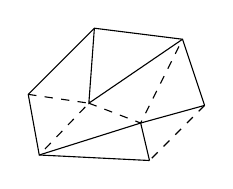
\begin{tikzpicture}[scale=1.4]
\draw (-.60,.10)--(0,.70)--(.80,.60)--(1,0);
\draw (.50,-.50)--(-.50,-.45)--(-.60,.10);
\draw[dashed] (1,0)--(.50,-.50);
\draw (0,.70)--(-.05,.02)--(.80,.60);
\draw (-.50,-.45)--(.42,-.16)--(1,0);
\draw (.42,-.16)--(.50,-.50);
\draw[dashed] (-.60,.10)--(-.05,.02)--(-.50,-.45);
\draw[dashed] (-.05,.02)--(.42,-.16)--(.80,.60);
\end{tikzpicture}
}
\par\noindent\textit{Typed diagram explanation: the source polygon is divided by solid and dashed segments into a proposed triangulation. The lecture explicitly permits attaching handles; the picture does not specify every global identification.}\par

(attaching handles is allowed!)
(A simplicial complex of a given genus) $f_k^{2n}(g)$ (Bessis).
(Number of triangulations \EnglishIncomplete{GELFAND-P001353}{cancel-bottom-word}{an undeciphered crossed-out word} of a surface of genus $g$ with $k$ triangles, [continuation below on the left:] $2n$-gons)



\par\smallskip\noindent\textit{Reading notes.}\par
\noindent\texttt{GELFAND-0146-U016} (cancel-21): A final single symbol after the crossed-out F(x,t), before (21).\par
Candidates: =; an unidentified single symbol. Unresolved in the frozen transcription.\par
\noindent\texttt{GELFAND-0146-U017} (cancel-variant-line): Beneath the question about the 2n-gon, “Number” is crossed out, followed by a short abbreviation with a loop and an ending resembling “kl”.\par
Candidates: gluings (abbreviated). Unresolved in the frozen transcription.\par
\noindent\texttt{GELFAND-0146-U018} (cancel-bottom-word): A crossed-out word between “triangulations” and “surface of genus g” in the bottom line.\par
Candidates: none. Unresolved in the frozen transcription.\par
The localized cancelled writing remains undeciphered. The frozen source frame remains partly unreadable; translating this note does not decipher the missing writing.\par
\noindent\texttt{GELFAND-0146-U019} (asympt-word): A joined word between “here” and “asymptotics”; its beginning and several middle strokes cannot be separated.\par
Candidates: most; interested (abbreviated). Unresolved in the frozen transcription.\par


\EnglishSourceFrame{GELFAND-P001354}{87}
(1971--79, Itzykson et al.)
\tikz{\node[draw,circle,inner sep=1pt] {2};}
\EnglishDiagramPair{GELFAND-P001354}{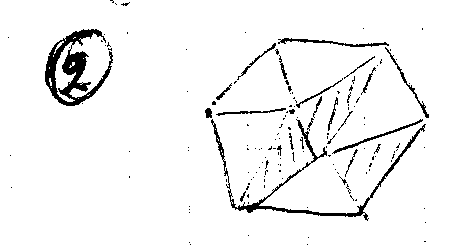
\includegraphics[width=.98\linewidth,height=45mm,keepaspectratio]{english/reader-working/chapter29-batch01/figures/gelfand-0146-d12-gelfand-p001354-original.png}}{
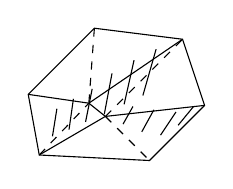
\begin{tikzpicture}[scale=1.4]
\draw (-.60,.10)--(0,.70)--(.80,.60)--(1,0)--(.50,-.50)--(-.50,-.45)--(-.60,.10);
\draw[dashed] (0,.70)--(-.05,.02);
\draw (-.05,.02)--(.80,.60);
\draw (-.50,-.45)--(.10,-.10)--(1,0);
\draw (-.60,.10)--(-.05,.02)--(.10,-.10);
\draw[dashed] (.10,-.10)--(.50,-.50);
\draw[dashed] (.10,-.10)--(.80,.60);
\draw[dashed] (-.50,-.45)--(-.05,.02);
\draw (-.38,-.28)--(-.34,-.03);
\draw (-.23,-.22)--(-.19,.06);
\draw (-.08,-.15)--(-.02,.15);
\draw (.09,-.08)--(.16,.29);
\draw (.27,.01)--(.36,.41);
\draw (.44,.09)--(.56,.51);
\draw (.26,-.17)--(.35,-.01);
\draw (.43,-.24)--(.54,-.04);
\draw (.60,-.27)--(.74,-.06);
\draw (.76,-.18)--(.90,-.01);
\end{tikzpicture}
}
\par\noindent\textit{Typed diagram explanation: the source retains the polygon division and hatches selected regions. The admitted correction makes the upper-left interior segment dashed. The accompanying text specifies white and black coloring and a fixed boundary gluing.}\par

The same, but we color and fix the gluing of the boundary; \EnglishUnclear{GELFAND-P001354}{boundary-short-word}{color.? [abbreviation uncertain]} white and black.



\par\smallskip\noindent\textit{Reading notes.}\par
The boundary abbreviation remains uncertain. The upper-left interior segment is dashed in the admitted source correction; the other geometry is inherited.\par


\EnglishSourceFrame{GELFAND-P001355}{unlabelled}
\underline{9/III--87.} Gelfand seminar.
\underline{I. M. G.} There is a paper which says the following; consider
\begin{equation*}
z\longmapsto\frac{\alpha z+\beta}{\gamma z+\delta},\qquad
\alpha,\beta,\gamma,\delta\in\mathbb Z,
\end{equation*}
[Crossed out after $\mathbb Z$: \EnglishUnclear{GELFAND-P001355}{cancel-after-z}{a short unreadable mathematical expression}.]
in the half-plane $\operatorname{Im}z>0$; $\alpha\delta-\gamma\beta>0$.
[Crossed out before There exist: \EnglishUnclear{GELFAND-P001355}{cancel-before-exists}{in kr-ve? [abbreviation undeciphered]}.]
There exist sets of nonzero intermediate Hausdorff measure,
which arise in connection with the \underline{principal series}.

\underline{Conjecture}: factors arise in representations of $\infty$-dimensional groups.
In physics, factors arise of type $\overline{III}_{\infty}$,
among them, exactly 1 hyperfinite [source abbreviation].

\underline{\EnglishUnclear{GELFAND-P001355}{list-heading}{Talkativeness? / ailments? [heading not established]}}:
a) factors;
b) attractors; c) chaos; Hausdorff measures and infin\EnglishUnclear{GELFAND-P001355}{list-series}{ite? [terminal letter uncertain]} series;
d) characteristic functions.

\underline{A. Beilinson.}
\underline{Basic facts about the Riemann $\zeta$-function and its generalizations.}
\begin{equation*}
\zeta(s)=\sum_{n=1}^{\infty}\frac1{n^s}.
\end{equation*}
1. Euler product:
\begin{equation*}
\zeta(s)=\prod_p(1-p^{-s})^{-1}.
\end{equation*}
2. Analytic continuation: a simple pole at $s=1$; holomorphic at the other points.

3. Functional equation. Introduce also the following $\zeta$-function:
\begin{equation*}
\zeta^*(s)=\underbrace{\pi^{-s/2}\Gamma(s/2)}_{\text{Euler factor numbered }\infty}\zeta(s),
\end{equation*}
Then $\zeta^*(s)$ is invariant under the substitution $s\to1-s$.
(unlike the $p$-metric)

[In the left margin: \underline{Remark 1.} \underline{Kirillov's}.]
\EnglishUnclear{GELFAND-P001355}{bottom-prefix}{$\pi$ / $\Pi$}
[Crossed out: \EnglishUnclear{GELFAND-P001355}{bottom-cancel}{a short unreadable symbol}.]
factor is the volume of an $s$-dimensional ball.



\par\smallskip\noindent\textit{Reading notes.}\par
\noindent\texttt{GELFAND-0146-U021} (cancel-after-z): Immediately after Z, a short dense group of mathematical strokes is crossed out.\par
Candidates: none. Unresolved in the frozen transcription.\par
\noindent\texttt{GELFAND-0146-U022} (cancel-before-exists): Before “There exist”, short crossed-out writing resembles “v kr-ve”.\par
Candidates: v kr-ve (unexpanded abbreviation); v k-ve (unexpanded abbreviation). Unresolved in the frozen transcription.\par
\noindent\texttt{GELFAND-0146-U023} (physics-ending): At the complete end of the line, “exactly 1” is readable, followed by a word resembling “continuity”; the ending remains qualified in the frozen record.\par
Candidates: exactly 1 continuity?. Unresolved in the frozen transcription.\par
The root-admitted literal correction reads “exactly 1 hyperfinite” (the source adjective is abbreviated). It replaces only the old uncertain reading; no factor classification is repaired.\par
\noindent\texttt{GELFAND-0146-U024} (list-heading): The underlined list heading begins “Zabol...”; its ending is joined.\par
Candidates: ailments? [nonstandard heading, tentative]. Unresolved in the frozen transcription.\par
The admitted candidate retains two uncertain surfaces: Zaboltennosti? / Zaboleznennosti?. The English gloss “Talkativeness? / ailments?” is tentative, not a resolved heading.\par
\noindent\texttt{GELFAND-0146-U025} (list-first-word): In item a), the word begins “frakt...” with a lower stroke and an ending resembling “ory”.\par
Candidates: fraktory? [nonstandard word]; fractals?. Unresolved in the frozen transcription.\par
The root-admitted literal correction reads “factors”; this is the active English translation.\par
\noindent\texttt{GELFAND-0146-U026} (bottom-prefix): Before the crossed-out symbol and “factor”, two vertical strokes have a connection at the top.\par
Candidates: pi; Pi. Unresolved in the frozen transcription.\par
\noindent\texttt{GELFAND-0146-U027} (bottom-cancel): Between the initial symbol and “factor”, a short symbol lies beneath diagonal strokes.\par
Candidates: none. Unresolved in the frozen transcription.\par
\noindent\texttt{GELFAND-0146-U034} (list-series): At the end of item c), an abbreviation precedes “series”; the initial loops and middle connections are ambiguous.\par
Candidates: principal series; infinite series. Unresolved in the frozen transcription.\par
The admitted source reads “bes” followed by uncertain “k.?” before “series”; translated as “infin[ite?] series”, retaining the uncertain ending.\par
\noindent\texttt{GELFAND-0146-U035} (bottom-word): After “factor”, a word visibly begins “sem...”; its ending and reading have not been established in the frozen record.\par
Candidates: families?; family?; layer?. Unresolved in the frozen transcription.\par
The admitted literal correction reads “volume of an s-dimensional ball”; the old family/layer candidates remain historical only.\par


\EnglishSourceFrame{GELFAND-P001356}{unlabelled}
\begin{equation*}
\mathbb R^*\qquad t^{-s}\qquad e^{-t^2}.
\end{equation*}
$\Gamma$ arises as a Mellin transform.
\begin{equation*}
\mathbb Q_p^*\qquad |t|^s\qquad\underbrace{\text{characteristic function of }(\mathbb Z_p\setminus0)}_{\text{open subgroup}}\subset\mathbb Q_p^*.
\end{equation*}
its analogue in $\mathbb R^*$ \EnglishUnclear{GELFAND-P001356}{analogue-abbrev}{ud.? / decreasing? [abbreviation uncertain]} of a Gaussian \underline{exp}.

4. Trivial zeros: the functional equation makes it clear that $\zeta(s)$ has zeros
(of multiplicity 1) at $s=-2k$, $k\in\mathbb Z$, $k>0$ (because of the $\Gamma$ factor).
[A short crossed-out group below: \EnglishUnclear{GELFAND-P001356}{cancel-under-four}{a short unreadable crossed-out group}.]

5. Rational values:
\begin{equation*}
\zeta(1-n)=-\frac{B_n}{n}.
\end{equation*}
(at negative points)
[Crossed out before $(t\,d/dt)^n$: \EnglishUnclear{GELFAND-P001356}{cancel-before-derivative}{a short unreadable crossed-out group}.]
\begin{equation*}
\zeta(-n)=\sum k^n=\left.\left(t\frac d{dt}\right)^n\frac1{1-t}\right|_{t=1}\qquad\star.
\end{equation*}
(more precisely, take the value of the first regular term)

6. Regulator formulas: $\forall n$, $\exists$ a natural subgroup in $\mathbb R$,
$\Gamma_n\subset\mathbb R$, such that
[Crossed-out line: $\zeta(1-2n)=(\operatorname{vol}\mathbb R/\Gamma_n)\cdot(\text{rational number})$.]
\begin{equation*}
\zeta'(-2n)=(\operatorname{vol}\mathbb R/\Gamma_n)\cdot(\text{rational number}).
\end{equation*}
$\Gamma_n$ is the image of $K_{4n+1}(\mathbb Z)$ in $\mathbb R$.

7. Arithmetic properties of Bernoulli numbers: $p$-adic properties of $\zeta(1-n)$.
\begin{equation*}
\zeta(s)(1-p^{-s})
\end{equation*}
\begin{equation*}
\zeta(1-n)(1-p^{-1+n})=\int_{\mathbb Z_p^*}x^{1-n}\,d\mu,
\end{equation*}
where $d\mu$ is a natural measure on $\mathbb Z_p^*$ (with values in $\mathbb Z_p$).
[Crossed out to the left of the next line: \EnglishUnclear{GELFAND-P001356}{cancel-left-units}{a symbol resembling E}.]
\begin{equation*}
\mathbb Z_p^*=(1+p\mathbb Z_p)\times\sqrt[p-1]{1},\qquad ((p-1)\text{th roots}).
\end{equation*}
The set of characters \EnglishUnclear{GELFAND-P001356}{character-word}{sil? [undeciphered word]} $\mathbb Z_p^*$ consists of $(p-1)$ components.

8. Riemann hypothesis.

9. Connection with the distribution of prime numbers.


\par\smallskip\noindent\textit{Reading notes.}\par
\noindent\texttt{GELFAND-0146-U029} (analogue-abbrev): Between R* and “Gaussian”, a short abbreviation consists of two symbols and a full stop.\par
Candidates: ud. [unexpanded abbreviation]; decreasing (abbreviated). Unresolved in the frozen transcription.\par
\noindent\texttt{GELFAND-0146-U030} (cancel-under-four): Beneath item 4, a short crossed-out group has overlapping strokes; the exact number of symbols has not been established.\par
Candidates: none. Unresolved in the frozen transcription.\par
\noindent\texttt{GELFAND-0146-U031} (cancel-before-derivative): Before the derivative, a short group is crossed out; the exact number of original symbols has not been established.\par
Candidates: none. Unresolved in the frozen transcription.\par
\noindent\texttt{GELFAND-0146-U032} (cancel-left-units): To the left of the decomposition of Z\_p*, a vertical symbol has three short strokes and a diagonal cancellation stroke.\par
Candidates: E. Unresolved in the frozen transcription.\par
\noindent\texttt{GELFAND-0146-U033} (character-word): Between “characters” and Z\_p*, three joined symbols resemble “sil”.\par
Candidates: sil [unexpanded uncertain word]. Unresolved in the frozen transcription.\par


\EnglishSourceFrame{GELFAND-P001357}{91}
% Historical transcription provenance: original PNG 2408 x 3448 viewed directly; no OCR used.
% Historical coordinates: (left, top, right, bottom), original pixels, origin (0,0)
% at the upper left; right and bottom limits excluded.
% Historical scales refer to viewing only; they supply no new source pixels.
% review top-heading: bbox=(205, 25, 1110, 140); nearest-neighbour x3
% review top-definition: bbox=(185, 140, 1150, 430); nearest-neighbour x3
% review euler-product: bbox=(280, 430, 1670, 600); nearest-neighbour x3
% review closure-line: bbox=(175, 585, 2160, 795); nearest-neighbour x2
% review embedding-line: bbox=(185, 755, 1355, 900); nearest-neighbour x3
% review invariance: bbox=(255, 890, 1950, 1010); nearest-neighbour x3
% review inertia-heading: bbox=(235, 1000, 950, 1260); nearest-neighbour x3
% review trivial-action: bbox=(350, 1250, 1230, 1430); nearest-neighbour x3
% review rings-diagram: bbox=(1380, 1030, 2080, 1435); nearest-neighbour x3
% review inertia-diagram: bbox=(175, 1410, 1380, 1830); nearest-neighbour x2
% review frobenius-note: bbox=(1010, 1640, 2075, 1990); nearest-neighbour x3
% review ramification: bbox=(210, 1950, 2000, 2215); nearest-neighbour x3
% review bibliography: bbox=(180, 2210, 1730, 2360); nearest-neighbour x3
% review local-factor: bbox=(235, 2340, 1330, 2500); nearest-neighbour x3
% review example1-heading: bbox=(180, 2480, 1080, 2620); nearest-neighbour x3
% review example1-text: bbox=(195, 2580, 2200, 2750); nearest-neighbour x3
% review galois-character: bbox=(195, 2730, 1310, 3010); nearest-neighbour x3
% review dirichlet-series: bbox=(275, 2990, 1660, 3265); nearest-neighbour x3
% review inertia-margin: bbox=(180, 1605, 455, 1840); nearest-neighbour x6
% review frobenius-leader: bbox=(995, 1680, 1195, 1850); nearest-neighbour x7
% review cancellations-top: bbox=(415, 240, 525, 410); nearest-neighbour x8
% review cancellations-closure: bbox=(195, 610, 455, 810); nearest-neighbour x6
% review ramification-word: bbox=(590, 1970, 790, 2065); nearest-neighbour x6
% review ramification-ending: bbox=(1575, 1955, 1930, 2065); nearest-neighbour x5
% review inertia-margin-text: bbox=(195, 1615, 400, 1745); nearest-neighbour x8
% review inertia-root: bbox=(305, 1660, 396, 1773); nearest-neighbour x10
% review bibliography-title: bbox=(1030, 2215, 1730, 2345); nearest-neighbour x4
% review sum-index: bbox=(510, 3120, 741, 3225); nearest-neighbour x7
% review galois-character-verb: bbox=(510, 2738, 1145, 2845); nearest-neighbour x4
% review embedding-arrow: bbox=(928, 780, 1053, 859); nearest-neighbour x9
% review compare-field-word: bbox=(890, 592, 1090, 704); nearest-neighbour x6
% review inertia-margin-final: bbox=(182, 1518, 450, 1845); nearest-neighbour x4
% review page-label: bbox=(2230, 46, 2384, 198); nearest-neighbour x5
% review almost-all-compare: bbox=(785, 1948, 979, 2072); nearest-neighbour x6
% review lower-border: bbox=(0, 3230, 2408, 3448); nearest-neighbour x1

\underline{Generalizations of the Riemann $\zeta$-function.}

$L$-functions of Artin \quad $L(\rho,s)$

\begin{equation*}
\rho:\operatorname{Gal}\overline{\mathbb{Q}}/\mathbb{Q}
\underset{\text{continuous}}{\longrightarrow} GL(n,\mathbb{C})
\end{equation*}
[Crossed out between $\operatorname{Gal}$ and $\overline{\mathbb{Q}}/\mathbb{Q}$:
\EnglishUnclear{GELFAND-P001357}{cancellation-galois}{illegible symbols}.]

\begin{equation*}
L(\rho,s)=\prod_p L_p(\rho,s),\qquad p\text{ is a prime number}
\end{equation*}

[Crossed out:
\EnglishUnclear{GELFAND-P001357}{cancellation-closure-word}{an illegible word}.]
$\overline{\mathbb{Q}}_p$ is an algebraic closure of the field $\mathbb{Q}_p$; fix an embedding
$\overline{\mathbb{Q}}\subset\overline{\mathbb{Q}}_p\quad\Rightarrow$

[Crossed out beneath the start of the line:
\EnglishUnclear{GELFAND-P001357}{cancellation-closure-formula}{$\mathbb{Q}_p/\mathbb{Q}$ or $\overline{\mathbb{Q}}_p/\mathbb{Q}$}.]

$\Rightarrow$ an embedding
$\operatorname{Gal}\overline{\mathbb{Q}}_p/\mathbb{Q}_p
\hookrightarrow\operatorname{Gal}\overline{\mathbb{Q}}/\mathbb{Q}$

Only the conjugacy class of these maps is invariantly determined.

Inertia group:
\begin{equation*}
I\hookrightarrow\operatorname{Gal}\overline{\mathbb{Q}}_p/\mathbb{Q}_p
\end{equation*}
acts trivially on $\overline{\mathbb{F}}_p=\overline{\mathbb{Z}/p\mathbb{Z}}$

% Right diagram: no visible arrow joins the upper right vertex;
% the original has no vertical arrows between rows.
\begin{center}
\begin{tikzcd}[column sep=large,row sep=large]
\overline{\mathbb{Z}/p\mathbb{Z}} &
\overline{\mathbb{Z}}_p \arrow[l] &
\overline{\mathbb{Q}}_p \\
\mathbb{Z}/p\mathbb{Z} &
\mathbb{Z}_p \arrow[l] \arrow[r,hook] &
\mathbb{Q}_p
\end{tikzcd}
\end{center}
\par\noindent\textit{Typed diagram explanation: the right-hand ring diagram has the arrows exactly as drawn: the middle entry maps left in each row, and $\mathbb Z_p$ embeds right into $\mathbb Q_p$. No upper-right or vertical arrow has been added.}\par


\begin{center}
\begin{tikzcd}[column sep=large,row sep=large]
I \arrow[r,hook] &
\operatorname{Gal}\overline{\mathbb{Q}}_p/\mathbb{Q}_p
  \arrow[r,hook] \arrow[d] &
\operatorname{Gal}\overline{\mathbb{Q}}/\mathbb{Q} \\
& \operatorname{Gal}\overline{\mathbb{Z}/p\mathbb{Z}}=\widehat{\mathbb{Z}} &
\end{tikzcd}
\end{center}
\par\noindent\textit{Typed diagram explanation: the second diagram embeds $I$ into the local Galois group and that group into the global Galois group. Its downward arrow goes to the Galois group of the algebraic closure of the residue field, written as $\widehat{\mathbb Z}$.}\par


[In the left margin, a callout to $I$:] leaves fixed $\sqrt[N]{1}$,
$(N,p)=1$

\EnglishDiagramPair{GELFAND-P001357}{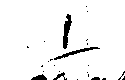
\includegraphics[width=12mm,keepaspectratio]{english/reader-working/chapter29-batch01/figures/mark-native-proof.png}}{
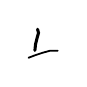
\begin{tikzpicture}[x=0.24pt,y=-0.24pt,line cap=round,line join=round]
\draw[line width=1.1pt] (64.5,47.5)--(65.5,38.0)--(68.0,28.0)--(70.0,21.0)--(68.5,15.5);
\draw[line width=0.65pt] (55.0,58.5)--(64.0,55.0)--(76.0,51.0)--(87.0,48.0)--(99.0,48.0);
\end{tikzpicture}
}
\EnglishSourceFigure{GELFAND-P001357}{frobenius-mark}{Below $\widehat{\mathbb{Z}}$, before the word ``generator'', there is a short vertical stroke above a slanted line: possibly an underlined $1$, possibly a callout mark. The two strokes are separate; their literal identity remains uncertain.}

generator $\mathrm{Fr}_p$ (Frobenius element $x\mapsto x^p$)

$\rho$ continuous $\Rightarrow$ for almost all $p$, except finitely many,
$\rho|_I$ is trivial.

Unramified $p$: $\rho(I_p)=1$

\underline{Literature:} \underline{Cassels, Fr\"ohlich} ``Algebraic Number Theory''

\begin{equation*}
L_p(\rho,s)=\det\bigl(1-\rho(\mathrm{Fr}_p)p^{-s}\bigr)^{-1}
\end{equation*}

\underline{Example 1.} Dirichlet $L$-functions

$\rho$: 1-dimensional representations defined by Dirichlet characters
$\chi:(\mathbb{Z}/N\mathbb{Z})^*\longrightarrow\mathbb{C}^*$

From it, a character of the Galois group is constructed
\begin{equation*}
\operatorname{Gal}\overline{\mathbb{Q}}/\mathbb{Q}
\longrightarrow (\mathbb{Z}/N\mathbb{Z})^*
\overset{\chi}{\longrightarrow}\mathbb{C}^*
\end{equation*}

\begin{equation*}
L(\chi,s)=\sum_{(n,N)=1}\frac{\chi(n)}{n^s}
=\prod_{(p,N)=1}\bigl(1-\chi(p)p^{-s}\bigr)^{-1}
\end{equation*}



\par\smallskip\noindent\textit{Reading notes.}\par
\noindent\texttt{GELFAND-0147-U001} (cancellation-galois): Between Gal and Q-bar / Q, a vertical group is densely crossed out or overwritten; its lower strokes extend beneath the line. The original symbols cannot all be distinguished.\par
Candidates: none. Unresolved in the frozen transcription.\par
\noindent\texttt{GELFAND-0147-U002} (cancellation-closure-word): Before Q-bar with subscript p, at the beginning of the line about algebraic closure, a short word is covered by several horizontal cancellation strokes.\par
Candidates: none. Unresolved in the frozen transcription.\par
\noindent\texttt{GELFAND-0147-U003} (cancellation-closure-formula): Beneath the beginning of that line, large crossed-out symbols resemble two fields separated by a slash. The final symbol resembles Q, and the first may have subscript p. An overline on the first Q cannot be established.\par
Candidates: \textbackslash{}mathbb{Q}\_p/\textbackslash{}mathbb{Q}; \textbackslash{}overline{\textbackslash{}mathbb{Q}}\_p/\textbackslash{}mathbb{Q}. Unresolved in the frozen transcription.\par
\noindent\texttt{GELFAND-0147-U004} (frobenius-mark): Below Z-hat, above “generator”, there is a short almost vertical stroke and a separate slanted line beneath it. There is no clear arrowhead.\par
Candidates: underlined 1; a callout mark from Z-hat to “generator Fr\_p”. Unresolved in the frozen transcription.\par
The two separate strokes below the diagram may be an underlined 1 or a callout mark. They are not joined to the preceding diagram. All original ring-diagram arrows are preserved; no invisible arrow is supplied.\par


\EnglishSourceFrame{GELFAND-P001358}{unlabelled}
% Historical transcription provenance: original PNG 2408 x 3448 viewed directly; no OCR used.
% Historical coordinates: (left, top, right, bottom), original pixels, origin (0,0)
% at the upper left; right and bottom limits excluded.
% Historical scales refer to viewing only; they supply no new source pixels.
% review example2-heading: bbox=(230, 20, 1140, 285); nearest-neighbour x3
% review induced-text: bbox=(265, 280, 2200, 425); nearest-neighbour x3
% review induced-formula-left: bbox=(445, 405, 1265, 580); nearest-neighbour x3
% review dedekind-formula-right: bbox=(1200, 420, 2275, 730); nearest-neighbour x3
% review properties-top: bbox=(130, 650, 1410, 990); nearest-neighbour x3
% review product-property: bbox=(150, 980, 1210, 1140); nearest-neighbour x3
% review continuation: bbox=(270, 1140, 1220, 1340); nearest-neighbour x3
% review hypothesis: bbox=(220, 1335, 2150, 1605); nearest-neighbour x3
% review functional-equation: bbox=(190, 1625, 1525, 1880); nearest-neighbour x3
% review equation-note: bbox=(170, 1850, 1710, 2160); nearest-neighbour x3
% review continuation-first-words: bbox=(470, 1150, 1185, 1248); nearest-neighbour x4
% review hypothesis-parenthesis: bbox=(730, 1435, 1940, 1535); nearest-neighbour x3
% review epsilon-note-text: bbox=(790, 1890, 1695, 2000); nearest-neighbour x4
% review epsilon-arguments: bbox=(805, 1758, 1050, 1880); nearest-neighbour x8
% review final-line: bbox=(180, 2030, 760, 2150); nearest-neighbour x5
% review continuation-word: bbox=(493, 1147, 663, 1228); nearest-neighbour x8
% review parenthesis-word: bbox=(875, 1440, 1060, 1516); nearest-neighbour x8
% review page-label-area: bbox=(2130, 0, 2408, 340); nearest-neighbour x3
% review hypothesis-adjectives: bbox=(565, 1344, 1170, 1468); nearest-neighbour x4
% review parenthesis-context: bbox=(715, 1400, 1235, 1570); nearest-neighbour x4
% review parenthesis-whole-word: bbox=(910, 1440, 1135, 1538); nearest-neighbour x6
% review lower-frame: bbox=(0, 2110, 2408, 3448); nearest-neighbour x1

\underline{Example 2.} \quad $K/\mathbb{Q}\subset\overline{\mathbb{Q}}$

[In the upper right margin:]
\EnglishUnclear{GELFAND-P001358}{upper-right-mark}{a single vertical stroke; $1$?}

\begin{equation*}
\operatorname{Gal}\overline{\mathbb{Q}}/K
\subset\operatorname{Gal}\overline{\mathbb{Q}}/\mathbb{Q}
\end{equation*}

Take the induced representation; then the corresponding $L$-function is $\zeta_K(s)$

\begin{equation*}
\begin{aligned}
L(\operatorname{Ind}_{K/\mathbb{Q}},s)
&=\zeta_K(s)
=\prod_{\substack{p\text{ prime}\\\text{ideals in }K}}
\bigl(1-N(p)^{-s}\bigr)^{-1}\\
&=\sum_{\substack{\text{integral}\\\text{ideals }I\\\text{in }K}}N(I)^{-s}
\end{aligned}
\end{equation*}

\underline{Properties}

0. $L(\rho,s)$ uniquely determines $\rho$

! $K$ is \underline{\underline{not}} recovered from $\zeta_K(s)$

\begin{equation*}
L(\rho_1\oplus\rho_2,s)=L(\rho_1,s)L(\rho_2,s)
\end{equation*}

1. \underline{Analytic continuation}

$L$-functions \EnglishUnclear{GELFAND-P001358}{analytic-word}{of a field / almost all}
admit holomorphic continuation.

All admit meromorphic continuation

\underline{Conjecture.} $\forall$ irreducible nontrivial $\rho$:
$L(\rho,s)$ is holomorphic in $s$.

[Insertion beneath the line:]
(if \EnglishUnclear{GELFAND-P001358}{parenthetical-mark}{$\rho$ / a separate curved stroke}
\EnglishUnclear{GELFAND-P001358}{parenthetical-verb}{passed [source abbreviation; admitted reading]}
through $GL(n,\mathbb{C})$: an Artin function)

For $l$-adic representations, even meromorphicity is unknown

2. Functional equation. Known for Artin $L$-functions

\begin{equation*}
L^*(\rho,s)=\varepsilon(\rho s)L^*(\rho^*,1-s)
\end{equation*}
[Notation of the factor:
\EnglishUnclear{GELFAND-P001358}{epsilon-separator}{$\varepsilon(\rho s)$ / $\varepsilon(\rho,s)$}.]

[A square bracket underneath singles out $\varepsilon(\rho s)$; caption:]
an important $\mathrm{const}$ is contained here
(Gauss sums)

Trivial zeros, and so on.


\par\smallskip\noindent\textit{Reading notes.}\par
\noindent\texttt{GELFAND-0147-U005} (upper-right-mark): In the upper right margin, there is a small uneven vertical black stroke. No other symbols make a reliably readable leaf number with it.\par
Candidates: 1; nontextual stroke or blemish. Unresolved in the frozen transcription.\par
\noindent\texttt{GELFAND-0147-U006} (analytic-word): In the first line after “Analytic continuation”, between “L-functions” and “holomorphic”, a small group of letters is broken by gaps and dot-like marks. It permits either the joined word “of a field” or the abbreviation “almost all”.\par
Candidates: of a field; almost all. Unresolved in the frozen transcription.\par
\noindent\texttt{GELFAND-0147-U007} (parenthetical-mark): After “if”, below the insertion’s baseline, a short curved stroke resembles a shallow check mark. A complete loop that would securely identify rho is not visible.\par
Candidates: \textbackslash{}rho; a separate curved stroke. Unresolved in the frozen transcription.\par
\noindent\texttt{GELFAND-0147-U008} (parenthetical-verb): In the insertion “(if … through GL(n,C): an Artin function)”, the abbreviated word before “through” was read uncertainly in the frozen record. Its beginning resembles “pr”; on the right are a descending loop and several joined short strokes followed by a full stop. A long stroke from the line above enters its middle.\par
Candidates: passed (abbreviated). Unresolved in the frozen transcription.\par
The admitted literal correction reads “propushch.”. English “passed” preserves this abbreviated surface. “Factors through” would be a contextual mathematical paraphrase, which has not replaced the text.\par
\noindent\texttt{GELFAND-0147-U009} (epsilon-separator): In the functional-equation factor, no separate comma is discernible between rho and s. The visible writing has epsilon, an opening parenthesis, rho, s and a closing parenthesis; a printed rule on the paper runs through the intervening space.\par
Candidates: \textbackslash{}varepsilon(\textbackslash{}rho s); \textbackslash{}varepsilon(\textbackslash{}rho,s). Unresolved in the frozen transcription.\par
The upper-right stroke is not accepted as a page number. The analytic-continuation word and the separate curved stroke after “if” remain uncertain. The functional equation retains the visible factor without inserting a comma.\par
